% !TeX root = ../libro.tex
% !TeX encoding = utf8

\setchapterpreamble[c][0.75\linewidth]{%
	\sffamily
	Una vez hemos construido un algoritmo correcto, un paso importante es determinar su costo computacional, es decir, los recursos que necesita, tales como el tiempo o espacio. El análisis necesario para estimar estos costes es un problema teórico, para el cuál requeriremos de un marco formal, que definiremos al principio de este capítulo. \\
	Además veremos los costes de los algoritmos estudiados en el \autoref{ch:tercer-capitulo}. \\
	\par\bigskip
}
\chapter{Complejidad algorítmica}\label{ch:cuarto-capitulo}

Como ya mencionamos anteriormente, necesitamos un marco formal para estudiar la complejidad de un algoritmo, por ello utilizaremos la notación asintótica, que introducimos con las siguientes definiciones.

\begin{definicion}
	Dadas dos funciones $f,g:\mathbb{N}\rightarrow \mathbb{R}$ diremos que $f(n)=\Theta(g(n))$ si existen constantes $c_1,c_2$ y $n_0$ tales que $$0\leq c_1g(n)\leq f(n)\leq c_2g(n)\ \ \ \forall n\geq n_0.$$
\end{definicion}

\begin{definicion}
	Dadas dos funciones $f,g:\mathbb{N}\rightarrow \mathbb{R}$ diremos que $f(n)=O(g(n))$ si existen constantes $c$ y $n_0$ tales que $$0\leq f(n)\leq cg(n)\ \ \ \forall n\geq n_0.$$
\end{definicion}

\begin{definicion}
	Dadas dos funciones $f,g:\mathbb{N}\rightarrow \mathbb{R}$ diremos que $f(n)=\Omega(g(n))$ si existen constantes $c$ y $n_0$ tales que $$0\leq cg(n)\leq f(n)\ \ \ \forall n\geq n_0.$$
\end{definicion}

En esencia, la idea es establecer una cota para el crecimiento asintótico de una función a partir de otra, normalmente más simple. En particular, la notación $\Omega$ implica una cota inferior, $O$ una cota superior y $\Theta$ ambas. En la \autoref{fig:notacion_asintotica} podemos observar un ejemplo de cada tipo de notación. \\

\begin{figure}[!htb]
	\centering
	\begin{subfigure}{\linewidth}
		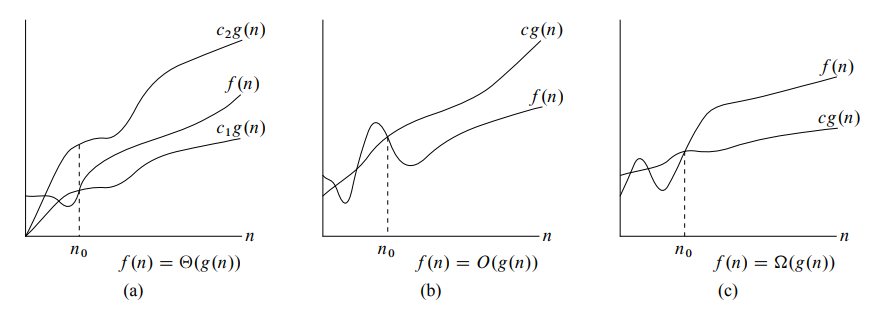
\includegraphics[width=14cm]{notacion_asintotica}
	\end{subfigure}
	
	\caption{Ejemplos gráficos de las notaciones $\Theta,O$ y $\Omega$. En cada imagen se muestra el valor mínimo para $n_0$, pero cualquier valor superior funciona también. Para el caso \textbf{(a)}, la notación $\Theta(g(n))$ implica una cota superior e inferior, por lo que la gráfica de $f(n)$ debe situarse entre las cotas obtenidas a partir de $g(n)$ y las constantes $c_1$ y $c_2$. En \textbf{(b)}, la notación $O(g(n))$ establece una cota superior, por lo que la gráfica de $f(n)$ se debe situar por debajo de la cota, obtenida a partir de la constante $c$. Por último, en \textbf{(c)} la notación $\Omega$ implica una cota inferior, luego en este caso, la gráfica de $f(n)$ debe de estar por encima de dicha cota, obtenida a partir de $c$. La imagen ha sido extraída de la referencia \cite{algorithms}, capítulo 3, figura 3.1.}
	\label{fig:notacion_asintotica}
\end{figure}

Utilizaremos la notación asintótica principalmente para describir el tiempo de ejecución de los algoritmos, pues es el recurso más importante, normalmente. Aunque también se suele estudiar el costo en espacio del algoritmo. \\

Cuando hablamos de tiempo de ejecución, hay que especificar de qué tiempo estamos hablando exactamente, pues existen varios interesantes. Entre otros, el tiempo medio de ejecución, el del peor caso, o el del mejor. Normalmente los datos más interesantes son el tiempo medio, pues es el tiempo de ejecución medio del algoritmo, y el tiempo de ejecución del peor caso, que establece un límite al tiempo máximo de ejecución del algoritmo. \\

Para poder analizar el tiempo de ejecución de un algoritmo de manera formal, tenemos que establecer un modelo de computación. En nuestro caso, supondremos que el computador tarda exactamente una unidad de tiempo en realizar cualquier instrucción básica, como pueden ser la suma, asignación, comparación, etc. Además, tomaremos como variables para medir el tiempo el tamaño del grafo de entrada, en concreto, el número de nodos y aristas. De esta manera, si decimos que un algoritmo es de orden $O(V)$ para un grafo $G=(V,E)$, nos referimos a que es lineal en el número de nodos. \\

A la hora de analizar los algoritmos estudiados, debemos tener en cuenta que en una cola normal, las operaciones \textbf{push()} y \textbf{pull()} son de orden $O(1)$, mientras que en una cola con prioridad, la operación \textbf{push()} es de orden $O(log(n))$ donde $n$ es el tamaño de la cola, y \textbf{pull()} es de orden $O(1)$. Nótese que estos órdenes son específicos para la librería estándar de C++ y podrían variar para otro lenguaje.

\section{Búsqueda en anchura}

Empezaremos por el algoritmo de Búsqueda en anchura (\autoref{BFS}). Primero tenemos que, debido a que cada vez que exploramos un nodo, lo marcamos como tal, y comprobamos que un nodo no haya sido explorado antes de proceder, las operaciones con la cola son de orden $O(V)$. Además, como itera sobre la lista de adyacencia de cada nodo sólo cuando es explorado, el algoritmo recorre cada lista de adyacencia una única vez. Como la suma de las longitudes de todas las listas de adyacencia es $\Theta(E)$, el tiempo gastado en escanear las listas es de $O(E)$. Por último, como el bucle de inicialización recorre una vez cada nodo, es de orden $O(V)$. Tenemos, en definitiva, que el algoritmo de búsqueda en anchura es de orden $O(V+E)$. Es decir, es lineal en el tamaño de la representación mediante listas de adyacencia de $G$.

\section{Dijkstra}

Continuamos con el algoritmo de Dijkstra (\autoref{DJK}). El análisis de este algoritmo es en esencia el mismo que el realizado para el algoritmo de búsqueda en anchura, pues la base del algoritmo es la misma. La única diferencia es el hecho de que utiliza colas con prioridad. Por esto, dado que la operación \textbf{push()} es de orden $O(log(V))$, y que esta operación se realiza dentro de los dos bucles principales del procedimiento, el orden final del algoritmo de Dijkstra es $O((V+E)log(V))$.

\section{Bellman-Ford}

Seguimos con el algoritmo de Bellman-Ford (\autoref{Bellman-Ford}). En este caso, el análisis es bastante simple, al ser un algoritmo muy corto. Primero, la operación de relajación es de orden $O(1)$, pues consta de comprobaciones y asignaciones. Ahora, por orden, la inicialización del algoritmo recorre todos los nodos del grafo, luego es de orden $O(V)$. A continuación tenemos dos bucles anidados, el primero recorre todos los nodos menos uno, y el segundo, por cada nodo, recorre todas las aristas. Este proceso es, por tanto, de orden $O(VE)$. El último bucle recorre todas las aristas realizando una comprobación, por lo que es de orden $O(E)$. En definitiva, el algoritmo de Bellman-Ford es de orden $O(VE)$.

\section{Algoritmo asociado a la multiplicación de matrices}

Analizaremos a continuación las dos versiones descritas en la \autoref{sec:3.4.1} asociadas a la multiplicación de matrices. Primero, el procedimiento $Extender_Caminos_Minimos(L,d)$, consta de tres bucles anidados, que realizan $n$ iteraciones cada uno, siendo $n$ el tamaño de la matriz de adyacencia, es decir, el número de nodos. El procedimiento es, por tanto, de orden $O(V^3)$. Ahora, la versión "Lenta" del algoritmo realiza este procedimiento dentro de un bucle una cantidad total de $n-2$ veces, luego es de orden $O(V)$, teniendo entonces un orden de $O(V^4)$ para la versión "Lenta" del algoritmo. La versión "Rápida" del algoritmo realiza el procedimiento $log_2(n)$ veces, gracias a los cálculos realizados en la descripción del algoritmo, siendo, por tanto, de orden $O(V^3log(V))$.

\section{Algoritmo de Floyd-Warshall}

Por último analizaremos la complejidad del algoritmo de Floyd-Warshall (\autoref{Floyd-Warshall}). Primero, el algoritmo base de Floyd-Warshall, que consta de tres bucles anidados que realizan cada uno $n$ iteraciones, siendo $n$ el tamaño de la matriz de adyacencia, es decir, el número de nodos. Puesto que las únicas operaciones que realiza el algoritmo son las de asignación, creación de matrices y la llamada a la función $min()$, todas de orden $O(1)$, el algoritmo es de orden $O(V^3)$. \\

El algoritmo completo, que calcula además los caminos, es idéntico en la parte de los tres bucles anidados, la única diferencia es que la operación de asignación donde se llamaba a la función $min()$, se ha sustituido por el condicional equivalente, que también es de orden $O(1)$. La parte que añade esta versión es la inicialización de la matriz $\Pi^(0)$, para la cuál se recorren todas las aristas del grafo. El orden del algoritmo es, por tanto, $O(V^3 + E) = O(V^3)$. Esta última igual es debida a que el número máximo de aristas en un grafo es $V(V-1)$, y, claramente, $V(V-1)<V^3$. \\

El algoritmo de la clausura transitiva tiene la misma estructura que la versión completa del algoritmo de Floyd-Warshall, luego es también de orden $O(V^3)$, aunque hay que destacar que el uso de variables booleanas hace que sea más rápido que el algoritmo principal.

\endinput



